\documentclass[12pt,letterpaper]{article}
\usepackage{fullpage}
\usepackage[top=2cm, bottom=4.5cm, left=2.5cm, right=2.5cm]{geometry}
\usepackage{amsmath,amsthm,amsfonts,amssymb,amscd}
\usepackage{lastpage}
\usepackage{enumerate}
\usepackage{fancyhdr}
\usepackage{mathrsfs}
\usepackage{xcolor}
\usepackage{graphicx}
\usepackage{listings}
\usepackage{hyperref}
\usepackage{fontspec,xunicode,xltxtra}
\usepackage{geometry}
\usepackage{xeCJK}
\usepackage{caption}
\usepackage{hyperref}
\usepackage{graphicx}
\setCJKmainfont{KaiTi}
%\setmainfont{Times New Roman}
\setCJKfamilyfont{hei}{SimHei}                                    %黑体  hei
\newcommand{\hei}{\CJKfamily{hei}}      

\hypersetup{%
  colorlinks=true,
  linkcolor=blue,
  linkbordercolor={0 0 1}
}
 
\renewcommand\lstlistingname{Algorithm}
\renewcommand\lstlistlistingname{Algorithms}
\def\lstlistingautorefname{Alg.}

\lstdefinestyle{Python}{
    language        = Python,
    frame           = lines, 
    basicstyle      = \footnotesize,
    keywordstyle    = \color{blue},
    stringstyle     = \color{green},
    breaklines      = true
    commentstyle    = \color{red}\ttfamily
}
\lstset{escapechar=@,style=Python}

\setlength{\parindent}{0.0in}
\setlength{\parskip}{0.05in}

% Edit these as appropriate
\newcommand\course{现代信息网络技术}
\newcommand\hwnumber{2}                  % <-- homework number
\newcommand\NetIDa{罗雁天}           % <-- NetID of person #1
\newcommand\NetIDb{2018310742}           % <-- NetID of person #2 (Comment this line out for problem sets)

\pagestyle{fancyplain}
\headheight 35pt
\lhead{\NetIDa}
\lhead{\NetIDa\\\NetIDb}                 % <-- Comment this line out for problem sets (make sure you are person #1)
\chead{\textbf{\Large Homework \hwnumber}}
\rhead{\course \\ \today}
\lfoot{}
\cfoot{}
\rfoot{\small\thepage}
\headsep 1.5em

\begin{document}

\section{发现两台服务器的IPv4地址和IPv6地址,以及对应的默认路由}
两台服务器的IPv4地址和IPv6地址如Table \ref{tab1}所示。
\begin{table}[!h]
	\centering
	\caption{\label{tab1}ee01服务器和ee02服务器的IPv4地址和IPv6地址}
	\begin{tabular}{|c|c|c|}
		\hline
		服务器地址 & IPv4地址 & IPv6地址 \\
		\hline
		ee01.cngi.edu.cn & 103.115.120.249/29 & 2402:e740:1:0:dff7:bbd9:abd5:3bb6/64\\
		\hline
		ee02.cngi.edu.cn & 103.115.120.250/29 & 2402:e740:1:0:e073:f075:555d:3bba/64\\
		\hline
	\end{tabular}
\end{table}

ee01服务器的默认路由为:
\begin{lstlisting}
default via 103.115.120.1 dev ens160 proto static metric 100 
103.115.120.1 dev ens160 proto static scope link metric 100 
103.115.120.248/29 dev ens160 proto kernel scope link src 103.115.120.249 metric 100 
\end{lstlisting}

ee02服务器的默认路由为:
\begin{lstlisting}
default via 103.115.120.1 dev ens160 proto static metric 100 
103.115.120.1 dev ens160 proto static scope link metric 100 
103.115.120.248/29 dev ens160 proto kernel scope link src 103.115.120.250 metric 100
\end{lstlisting}

\section{ping/ping6本端和另一个虚拟机的地址(10个报文、研究汇总报告)}
ee01服务器ping ee02服务器结果如Table \ref{tab2}所示:

\begin{table}[!h]
	\centering
	\caption{\label{tab2}ee01服务器ping ee02服务器的结果}
	\begin{tabular}{|c|c|c|c|c|c|c|}
		\hline
		地址类型 & ttl & packet loss & rtt min(ms) & rtt avg(ms) & rtt max(ms) & rtt mdev(ms) \\
		\hline
		IPv4地址 & 64 & 0\% & 0.073 & 0.099 & 0.238 & 0.047\\
		\hline
		IPv6地址 & 64 & 0\% & 0.074 & 0.095 & 0.208 & 0.039\\
		\hline
	\end{tabular}
\end{table}

ee02服务器ping ee01服务器结果如Table \ref{tab3}所示:
\begin{table}[!h]
	\centering
	\caption{\label{tab3}ee02服务器ping ee01服务器的结果}
	\begin{tabular}{|c|c|c|c|c|c|c|}
		\hline
		地址类型 & ttl & packet loss & rtt min(ms) & rtt avg(ms) & rtt max(ms) & rtt mdev(ms) \\
		\hline
		IPv4地址 & 64 & 0\% & 0.071 & 0.120 & 0.193 & 0.045\\
		\hline
		IPv6地址 & 64 & 0\% & 0.078 & 0.094 & 0.174 & 0.028\\
		\hline
	\end{tabular}
\end{table}

\section{找到你最喜欢的世界上的10所大学的网站,列出域名、对应的IPv4和IPv6地址,ping/ping6看到这些网站的延时和丢包率,traceroute/traceroute6看并总结路径的同异}
所涉及的大学网站、域名、IPv4地址和IPv6地址如Table \ref{tab6}所示
\begin{table}[!h]
	\centering
	\caption{\label{tab6}大学网站、域名、IPv4地址和IPv6地址表}
	\begin{tabular}{|c|c|c|c|}
		\hline
		高校名称 & 域名 & IPv4地址 & IPv6地址 \\
		\hline
		清华 & www.tsinghua.edu.cn & 166.111.4.100 & 2402:f000:1:404:166:111:4:100 \\
		\hline
		上海交大 & www.sjtu.edu.cn & 202.120.2.119 & 2001:da8:8000:1::2:119 \\
		\hline
		MIT & www.mit.edu & 23.2.132.180 & 2600:140e:6:388::255e \\
		\hline
		Stanford & www.stanford.edu & 52.2.93.140 & 无  \\
		\hline
		UCLA & www.ucla.edu & 164.67.228.152 & 2607:f010:2e8:228:0:ff:fe00:152 \\
		\hline
		UC Berkeley & www.berkeley.edu & 52.10.203.245 & 2600:1f14:436:7801:dcd1:212f:cfde:5ac3  \\
		\hline
		CMU & www.cmu.edu & 128.2.42.52 & 无 \\
		\hline
		Harvard & www.harvard.edu & 23.185.0.1 & 2620:12a:8001::1 \\
		\hline
		Columbia & www.columbia.edu & 28.59.105.24 & 无 \\
		\hline
		Yale(耶鲁) & www.yale.edu & 104.16.141.133 &2606:4700::6810:8d85 \\
		\hline
		Dartmouth & home.dartmouth.edu & 104.16.117.63 & 2606:4700::6810:763f \\
		\hline
		Brown & www.brown.edu & 104.17.84.62 & 2606:4700::6810:d925 \\
		\hline
		NYU & wustl.edu & 52.198.45.18 & 2607:f600:1002:6113::100 \\
		\hline
		Oxford & www.ox.ac.uk & 129.67.242.154 & 无 \\
		\hline
		Cambridge & www.cam.ac.uk & 128.232.132.8 & 无 \\
		\hline
	\end{tabular}
\end{table}


ping高校官网IPv4地址结果如Table \ref{tab4}所示,ping高校官网IPv6地址结果如Table \ref{tab5}所示,从中可以发现:
\begin{itemize}
	\item ping国内高校和国外高校的rtt的差据还是挺大的,国内网站的rtt小并且方差也小,国外网站的rtt大并且方差也大;
	\item 有些国外大学的官网使用ping6会出现“未知的名称或服务”的情况;
	\item 对NYU使用ping6命令结果正常,但是使用ping命令时丢包率却为100\%;
\end{itemize}
\begin{table}[!h]
	\centering
	\caption{\label{tab4}ee01服务器ping高校IPv4地址的结果}
	\begin{tabular}{|c|c|c|c|c|c|}
		\hline
		高校名称 & 域名 & ttl & packet loss & rtt avg(ms) & rtt mdev(ms) \\
		\hline
		清华 & www.tsinghua.edu.cn & 56 & 0\%& 0.808 & 0.076 \\
		\hline
		上海交大 & www.sjtu.edu.cn & 51 & 0\%& 25.979 & 0.161 \\
		\hline
		MIT & www.mit.edu & 47 & 0\% & 73.872 & 0.460 \\
		\hline
		Stanford & www.stanford.edu & 238 & 0\% & 384.333 & 11.812 \\
		\hline
		UCLA & www.ucla.edu & 48 & 0\% & 183.846 & 5.605\\
		\hline
		UC Berkeley & www.berkeley.edu & 232 & 0\% & 319.127 & 6.901 \\
		\hline
		CMU & www.cmu.edu & 239 & 0\% & 230.255 & 1.833 \\
		\hline
		Harvard & www.harvard.edu & 49 & 0\% & 319.334 & 21.511 \\
		\hline
		Columbia & www.columbia.edu & 232 & 0\% & 225.367 & 5.698 \\
		\hline
		Yale(耶鲁) & www.yale.edu & 49 & 0\% & 295.020 & 8.487 \\
		\hline
		Dartmouth & home.dartmouth.edu & 50 & 0\% & 281.822 & 6.884 \\
		\hline
		Brown & www.brown.edu & 50 & 0\% & 285.102 & 11.091 \\
		\hline
		Oxford & www.ox.ac.uk & 48 & 0\% & 232.646 & 0.314 \\
		\hline
		Cambridge & www.cam.ac.uk & 47 & 0\% & 235.644 & 0.536 \\
		\hline
	\end{tabular}
\end{table}

\begin{table}[!h]
	\centering
	\caption{\label{tab5}ee01服务器ping高校IPv6地址的结果}
	\begin{tabular}{|c|c|c|c|c|c|}
		\hline
		高校名称 & 域名 & ttl & packet loss & rtt avg(ms) & rtt mdev(ms) \\
		\hline
		清华 & www.tsinghua.edu.cn & 52 & 0\%& 0.997 & 0.123 \\
		\hline
		上海交大 & www.sjtu.edu.cn & 50 & 0\%& 25.866 & 0.178 \\
		\hline
		MIT & www.mit.edu & 53 & 0\% & 166.023 & 0.368 \\
		\hline
		UC Berkeley & www.berkeley.edu & 38 & 0\% & 187.189 & 2.666 \\
		\hline
		UCLA & www.ucla.edu & 48 & 0\% & 160.120 & 5.585\\
		\hline
		Harvard & www.harvard.edu & 48 & 0\% & 166.476 & 6.417 \\
		\hline
		Yale(耶鲁) & www.yale.edu & 52 & 0\% & 155.486 & 0.823 \\
		\hline
		Dartmouth & home.dartmouth.edu & 52 & 0\% & 160.496 & 5.288 \\
		\hline
		Brown & www.brown.edu & 52 & 0\% & 157.436 & 4.127 \\
		\hline
		NYU & wustl.edu & 35 & 0\% & 227.763 & 4.001 \\
		\hline
	\end{tabular}
\end{table}

使用traceroute查看路径可以发现,所有大学网站的路径中均有``42.247.33.65''这个地址,在同一地区的大学路由的路径中相同的地址较多,不同地区的大学路径中相同的地址较小。在北京之外的大学,路径中都经过了``101.4.113.217''这个地址,在此绘制出了其中几所高校官网的路由路径图如图\ref{res1}所示。

使用traceroute6查看路径可以发现,所有大学网站的路径前4跳均为``2402:e740:1::1'',``2001:da8:23d:1::1'',``2001:da8:257:0:101:4:1:102'',``2001:da8:257:0:101:4:113:6e'',并且清华和上交都经过了``2001:da8:2:701::1'',MIT、UC Berkeley、UCLA、Harvard、Yale都经过了``cernet2.net (2001:da8:a4:2::2)'',其中Harvard、UC Berkely和Yale还都经过了``cernet2.net (2001:252:0:302::2)
''。在此绘制出了其中几所高校官网的路由路径图如图\ref{res2}所示。

\begin{figure}[!h]
	\centering
	\begin{minipage}{\textwidth}
		\centering
		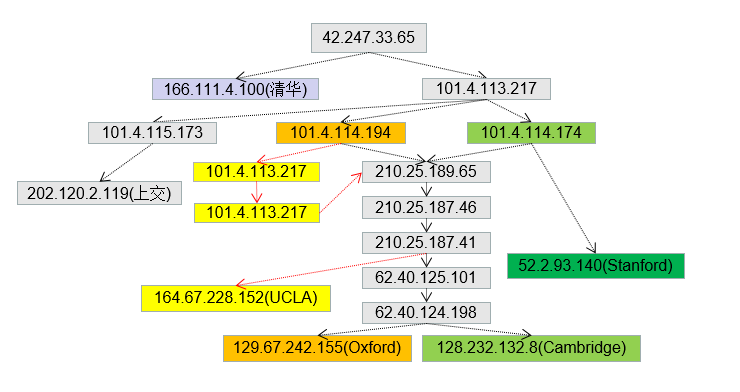
\includegraphics[width=\textwidth]{traceroute}
		\caption{\label{res1}高校官网的traceroute路径图}
	\end{minipage}
	\begin{minipage}{\textwidth}
		\centering
		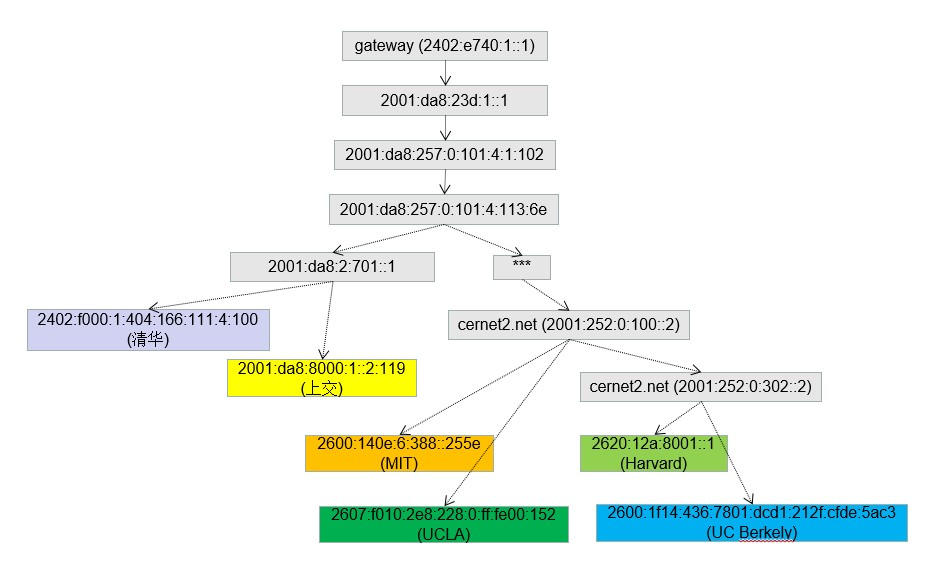
\includegraphics[width=\textwidth]{traceroute6}
		\caption{\label{res2}高校官网的traceroute6路径图}
	\end{minipage}
\end{figure}


\section{根据网上找到的IP地址库,分析每一跳的地址属性}
对于traceroute,我们在此分析到MIT官网的每一跳的地址属性如表\ref{tab7}所示。
\begin{table}[!h]
	\centering
	\caption{\label{tab7}ee01服务器traceroute到MIT官网每一跳的地址属性}
	\begin{tabular}{|c|p{11.8cm}|}
		\hline
		IPv4地址 & 属性 \\
		\hline
		42.247.33.65 & 亚洲,中国,北京,海淀,教育网,经度116.298,纬度39.959 \\
		\hline
		101.4.113.217 & 亚洲,中国,北京,教育网,经度116.405,纬度39.905 \\
		\hline
		101.4.116.14 & 亚洲,中国,北京,教育网,经度116.405,纬度39.905 \\
		\hline
		219.158.42.41 & 亚洲,中国,北京,联通/骨干网,经度116.405,纬度39.905 \\
		\hline
		219.158.5.129 & 亚洲,中国,北京,联通/骨干网,经度116.405,纬度39.905 \\
		\hline
		219.158.8.86 & 亚洲,中国,广东,广州,联通/骨干网,经度113.281,纬度23.125 \\
		\hline
		219.158.8.118 & 亚洲,中国,广东,广州,联通/骨干网,经度113.281,纬度23.125 \\
		\hline
		219.158.103.26 & 亚洲,中国,广东,广州,联通/骨干网,经度113.281,纬度23.126 \\
		\hline
		219.158.10.30 &  亚洲,中国,安徽,合肥,联通/骨干网,经度117.283,纬度31.861 \\
		\hline
		219.158.34.194 & 亚洲,中国,香港,联通/骨干网,经度114.173,纬度22.320 \\
		\hline
		*** & *** \\
		\hline
		23.13.184.222(www.mit.edu) & 亚洲,中国,香港,联通/骨干网,经度114.173,纬度22.320 \\
		\hline
	\end{tabular}
\end{table}

对于traceroute6,我们在此分析到MIT官网的每一跳的地址属性如表\ref{tab8}所示。
\begin{table}[!h]
	\centering
	\caption{\label{tab8}ee01服务器traceroute6到MIT官网每一跳的地址属性}
	\begin{tabular}{|c|p{10cm}|}
		\hline
		IPv6地址 & 属性 \\
		\hline
		2402:e740:1::1 & 中国 \\
		\hline
		2001:da8:23d:1::1 & 中国北京市 赛尔网络有限公司 \\
		\hline
		2001:da8:257:0:101:4:1:102 & 中国北京市 赛尔网络有限公司网络运行部 \\
		\hline
		2001:da8:257:0:101:4:113:6e &  中国北京市 赛尔网络有限公司网络运行部 \\
		\hline
		2001:252:0:100::2 & 中国 教育网(CNGI国际网,CNGIIGN) \\
		\hline
		2001:252:0:302::2 & 中国 教育网(CNGI国际网,CNGIIGN) \\
		\hline
		2001:470:0:2a2::1 & 美国California州Los Angeles Hurricane Electric, Inc. 骨干网 - Los Angeles - 中国CNGI国际网 (AS23911) \\
		\hline
		2001:504:13::210:65 & 美国Colorado州Denver 骨干交换网 - CoreSite \\
		\hline
		2403:e800:ff00:110::4d & 中国香港区 Telstra International Limited \\
		\hline
		2403:e800:218:5::2 & 中国香港区 Telstra International Limited \\
		\hline
		*** & *** \\
		\hline
		2600:140e:6:381::255e(www.mit.edu) & 美国 Akamai Technologies, Inc. \\
		\hline
	\end{tabular}
\end{table}
\end{document}
